\chapter{World Model and Scenario Description}

The scenario in this experiment consists of simulated worlds containing UAVs, moving targets, fixed targets, and target safe havens.  The UAVs work as a team to find all the targets and destroy them.  The simulated worlds are randomly generated via a custom utility for the project.  The number of UAVs, targets, and havens are configurable.  The worlds are rectangular and their sizes are configurable.  The utility reads the configuration file and generates data files describing random worlds.  See ~\ref{sec:exampleWorldCfg} for an example configuration file.

The direction of travel for moving targets is constrained to a randomly generated road network within the world.  The road network is created by randomly selecting a few seed locations within the world.  The locations are then used as the initial point set for constructing a \textit{k-d tree}(\cite{wiki:kdtree}).  A true \textit{k-d tree} is not constructed since the spatial partitioning bounds do not extend to infinity.  Instead the road construction algorithm simply keeps track of the location of the tree nodes and uses these as road intersections or corners.  See figures~\ref{fig:kdtree} and~\ref{fig:kdtreeroads} for a comparison between a typical \textit{k-d tree} partition and the simulated world road construction.  The \textit{k-d tree} algorithm was used for creating a road network since it mimics the geometric nature of urban streets.

\begin{figure}[h]
	\centering
	%\includegraphics[width=\linewidth,height=\textheight]{imagefile}
	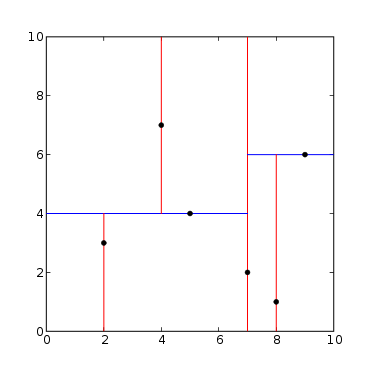
\includegraphics[scale=0.5]{370px-Kdtree_2d.png}
	%	\includegraphics{uav_monitor_states.png}
	\caption{Normal KD-Tree partitioning\protect\footnotemark}
	\label{fig:kdtree}
\end{figure}

\begin{figure}[h]
	\centering
	%\includegraphics[width=\linewidth,height=\textheight]{imagefile}
	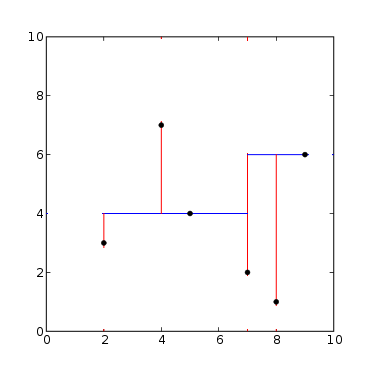
\includegraphics[scale=0.5]{Kdtree_roads.png}
	%	\includegraphics{uav_monitor_states.png}
	\caption{Simulation's KD-Tree roads}
	\label{fig:kdtreeroads}
\end{figure}

\footnotetext{A KD-Tree from the point set (2,3), (5,4), (9,6), (4,7), (8,1), (7,2).  Image from \url{https://en.wikipedia.org/wiki/File:Kdtree_2d.svg} and reused under the Creative Commons License}

``Target safe havens'' are locations in world where a target may flee to and be safe from UAV attack and surveillance.  These havens are randomly located within the world on the road network.  Moving targets will travel from one haven to the next.

When the simulation starts the UAVs begin searching the world for targets.  While scanning the world they update their internal belief model.  This internal model is shared with other members of the swarm when they are within communication's range of each other.  This model contains data regarding each UAV's confidence that a geographic region is clear and a list of known targets.  Section~\ref{sec:uavBelief} describes this model in detail.

When a target is found the UAV assigns an initial task status to the target and announces the discovery of the target.  The original UAV and anyone within range compute a scoring value to determine who is the most appropriate UAV to monitor and/or attack the target.  Soon after the other UAV's in range who heard the initial target announcement will re-broadcast their internal belief model's and therefore propagate the target discovery throughout the swarm.

\todo{Show a screenshot of the sim?}
